\chapter{Informationsgehalt und Entropie}
gedächtnislose Quelle mit Alphabet $\Omega$.\\
diskrete Zufallsvariable $X$ mit Werten $\Omega = \lbrace x_1,\ldots,x_m \rbrace$.\\\\
Auftrittswahrscheinlichkeiten:
\[ P(X=x_i) = p(x_i) \qquad \sum_{i=1}^{M} = 1 \]
~\\Informationsgehalt des Symbols $x_i$:
\[ I(x_i) = -\log_2p(x_i) \textrm{ bit} \]
~\\Entropie von $X$: mittlere Information pro Symbol:
\[ H(X) = \sum_{i=1}^{M}p(x_i)I(x_i) = -\sum_{i=1}^{M}p(x_i)\log_2p(x_i) \textrm{ bit} \]

\section{Maximaler Entscheidungsgehalt und Redundanz}
Die Entropie einer diskreten gedächtnislosen Quelle wird maximal,
wenn alle $M$ Symbole des Symbolvorrats gleich wahrscheinlich sind,
wenn also $p(x_i)=\frac{1}{M}$:
\[ H(X) = \log_2M \textrm{ bit} \]
~\\$H(X)$ kann als maximalen Entscheidungsgehalt eines aus $M$ Symbolen bestehenden
Symbolvorrats betrachtet werden.\\\\
Für eine beliebige Quelle gilt ($R$ = Redundanz der Quelle):
\[ R = \log_2M-H(X) \geq 0 \]

\section{Codierung}
natürliche Codierung:
\\Codewörter der Länge $n$, wobei $\log_2M \leq n < \log_2M+1$
\\\\
Quellencodierungstheorem (Shannon):
\\für jedes $\varepsilon > 0$ gibt es einen binären Präfix-Code mit Bitrate
\[ r_b \leq r_s \cdot H(X) + \varepsilon \]

\subsection{Huffman-Codierung}
\begin{enumerate}
	\item Ordnen: Zeichen nach fallenden Wahrscheinlichkeiten ordnen
	\item Reduzieren: Zeichen mit den zwei kleinsten WSK zusammenfassen,
		wieder zu 1.
	\item Codieren: Starten bei letzter Zusammenfassung; jeweils eine
		0 dem oberen Zweig, eine 1 dem unteren.
\end{enumerate}
\begin{center}
	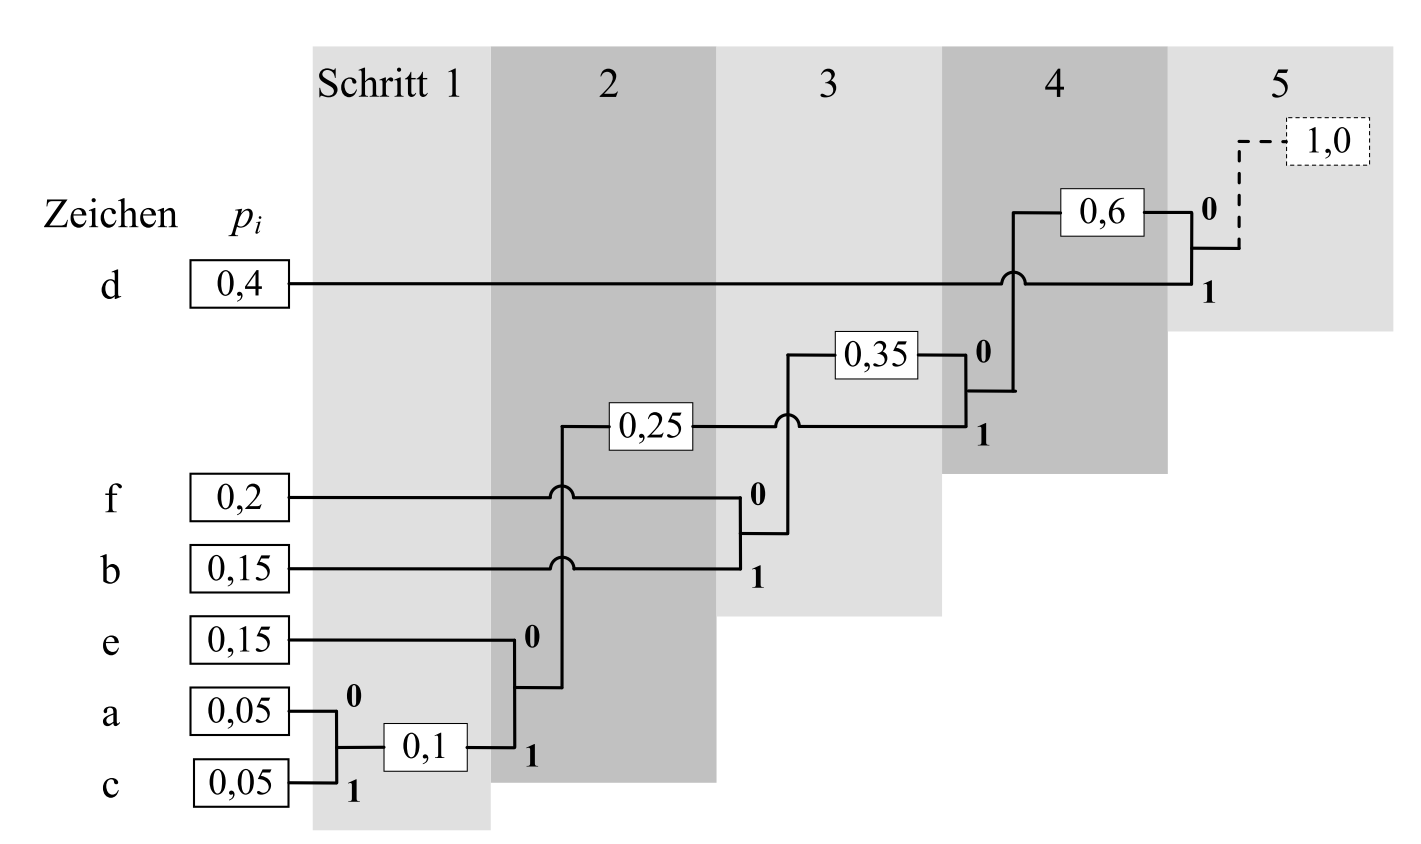
\includegraphics[width=.9\textwidth]{./images/huffman.png}
\end{center}
~\\
mittlere Codewortlänge:
\[ \bar{n} = \sum_{i=1}^{N}p_i \cdot n_i \]
~\\
Effizienz des Codes:
\[ \eta = \frac{H(X)}{\bar{n}} \]

\section{Bedingte Wahrscheinlichkeit}
Wahrscheinlichkeit von $y$ gegeben $x$:
\[ p(y|x) = \frac{p(x,y)}{p(x)} \]
~\\
Bedingter Informationsgehalt:
\[ I(y_j|x_i) = -\log_2p(y_j|x_i) \]
~\\
Wechselseitige Information des Symbolpaars ($x_i$,$y_j$) (Verbundquelle):
\[ I(x_i;y_j) = \log_2\frac{p(y_j|x_i)}{p(y_j)} = \log_2\frac{p(x_i|y_j)}{p(x_i)} \]
~\\
Informationsgehalt eines Symbolpaars:
\[ I(x_i,y_j) = I(x_i) + I(y_j) - I(x_i;y_j) \]
\[ I(x_i,y_j) = I(x_i) + I(y_j|x_i)  \]

\section{Verbundquellen}
Verbundentropie:
\[ H(X,Y) = - \sum_{i=1}^{M}\sum_{j=1}^{N} p(x_i,y_j)\log_2p(x_i,y_j) \]
~\\
bedingte Entropie:
\[ H(Y|X) = - \sum_{i=1}^{M}\sum_{j=1}^{N} p(x_i,y_j)\log_2p(x_i|y_j) \]

\begin{center}
	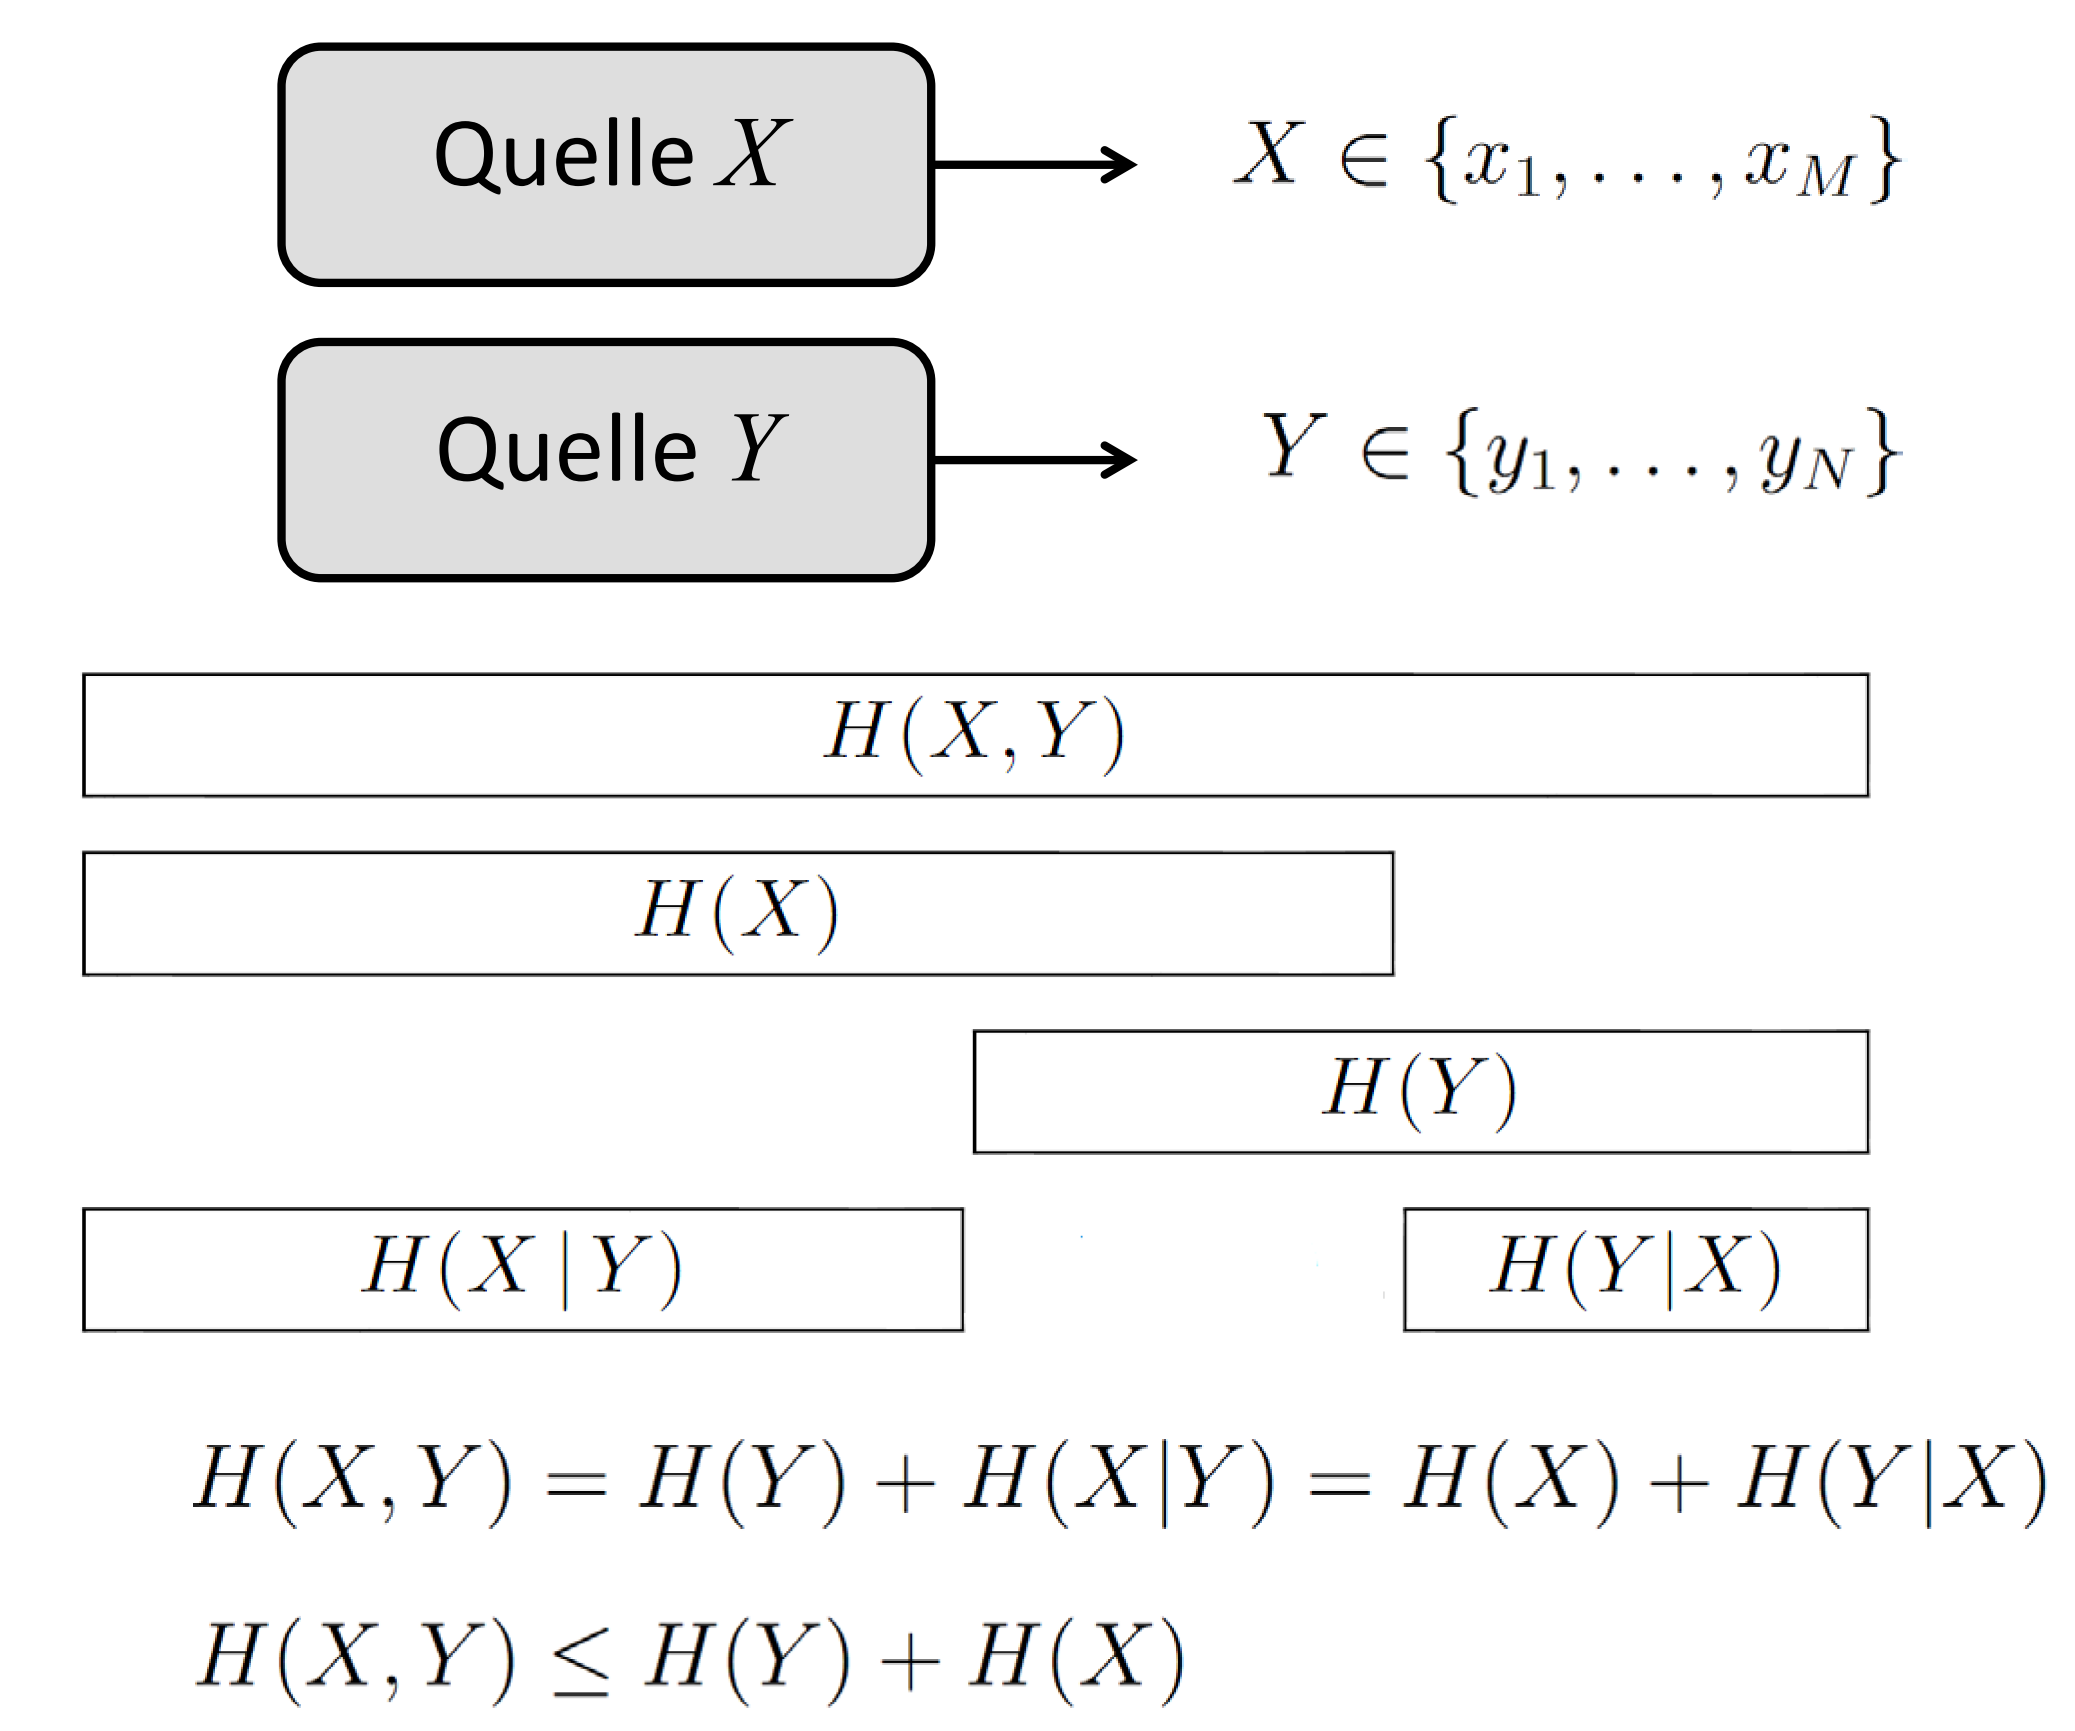
\includegraphics[width=.9\textwidth]{./images/verbundentro.png}
\end{center}

\section{Transinformation}
Transinfomration (mutual information):
\[ I(X;Y) = \sum_{i=1}^{M}\sum_{j=1}^{N}p(x_i,y_j)\log_2\frac{p(y_j|x_i)}{p(y_j)}
	= \sum_{i=1}^{M}\sum_{j=1}^{N}p(x_i,y_j)\log_2\frac{p(x_i|y_j)}{p(x_i)} \]
	
\begin{center}
	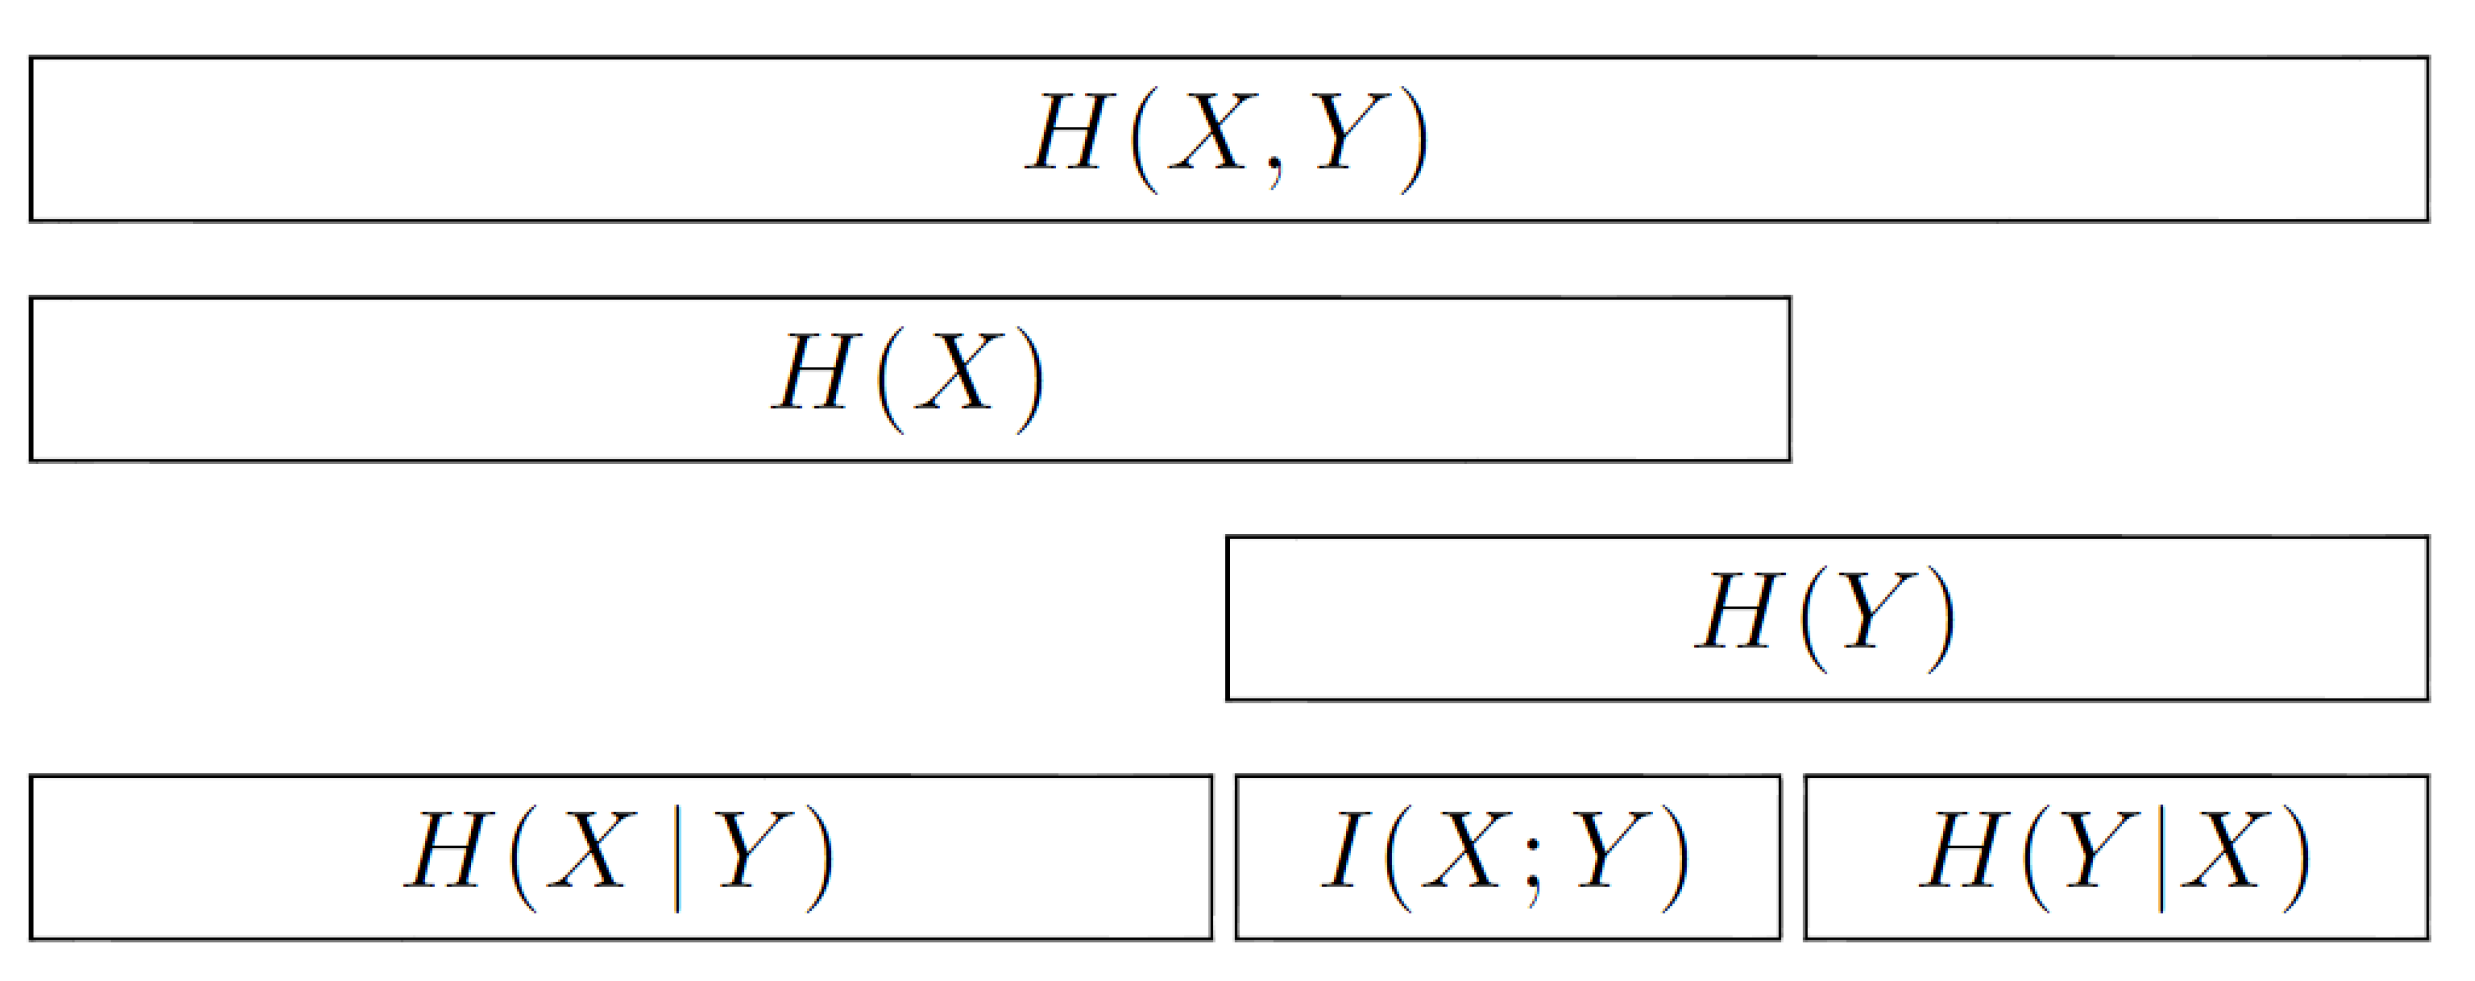
\includegraphics[width=.9\textwidth]{./images/transinfo.png}
\end{center}

\section{Kanalkapazität}
Die Kapazität eines Kanals entspricht der maximalen Transinformation des Kanals 
bei Speisung mit einer angepassten Quelle [bit/Kanalnutzung]:
\[ C = \max_X I(X;Y) \]
~\\
Bei symmetrischen diskreten gedächtnislosen Kanälen wird die Kanalkapazität 
durch eine Quelle mit Gleichverteilung erreicht. 
\\\\
kontinuierliche AWGN-Kanäle [bit/s]:
\[ C_{AWGN} = B\log_2\left(1+\frac{\bar{P}}{N_0 \cdot B}\right) \]
~\\
\begin{footnotesize}
\begin{tabular}{ll}
	$B$:	& Bandbreite \\
	$\bar{P}$:	& mittlere empfangene Signalleistung \\
	$N_0$:&	spektr. Rauschleistungsdichte
\end{tabular}
\end{footnotesize}